\documentclass[a4paper,12pt]{article}
\usepackage{times}
\usepackage[french]{babel}
\usepackage[utf8x]{inputenc}
\usepackage[T1]{fontenc}
\usepackage{amsmath}
\usepackage{amssymb}
\usepackage{graphicx}
\usepackage{pdfpages}
\usepackage{pdflscape}
\usepackage{listings}
\usepackage{longtable}
\lstset{literate=
{é}{{\'e}}1
{è}{{\`e}}1
{ê}{{\^e}}1
{à}{{\`a}}1
{â}{{\^a}}1
}
\lstset{language=C++,
                basicstyle=\footnotesize,
                keywordstyle=\footnotesize\color{blue},
                otherkeywords={override,nullptr}
}
\definecolor{orange}{rgb}{0.8,0.4,0.0}
\definecolor{darkblue}{rgb}{0.0,0.0,0.6}
\definecolor{cyan}{rgb}{0.0,0.6,0.6}
\lstdefinelanguage{JSON}
{
  basicstyle=\normalsize,
  columns=fullflexible,
  showstringspaces=false,
  commentstyle=\color{gray}\upshape,
  morestring=[b]",
  morestring=[s]{>}{<},
  morecomment=[s]{<?}{?>},
  stringstyle=\color{orange},
  identifierstyle=\color{darkblue},
  keywordstyle=\color{blue},
  morekeywords={string,number,array,object}% list your attributes here
}

\sloppy

\setlength{\topmargin}{0cm}
\setlength{\headsep}{0.in}
\setlength{\headheight}{0.in}
\setlength{\evensidemargin}{0cm}
\setlength{\oddsidemargin}{-1cm}
\textwidth 18cm
\textheight 25cm

\begin{document}

\thispagestyle{empty}

\begin{titlepage}

\vspace*{2cm}

\begin{center}\textbf{\Huge Projet Logiciel Transversal}\end{center}{\Large \par}

\begin{center}\textbf{\large Patrick Contin, William Duval Bourligueux, Bastien Guillard, Abdel-Oihed Houta}\end{center}{\large \par}

\vspace{2cm}

%\begin{figure}[h]
%\begin{center}
%\includegraphics[width=\textwidth]{exemple.png}
%\caption{\label{pacmangame}Exemple du jeu}
%\end{center}
%\end{figure}

\clearpage

{\small
\tableofcontents
}

\end{titlepage}

\clearpage
\section{Présentation Générale}

\subsection{Archétype}

Le jeu est un tactical RPG, basé sur des jeux tels que Final Fantasy
tactics, Fae tactics ou encore la série des Fire Emblem.

\subsection{Règles du jeu}

Le jeu se déroule sur une map la forme d'une grille, celle-ci voit 
s'affronter 2 équipes de plusieurs personnages. Chaque personnage peut se 
déplacer et interagir (attaquer, soigner, etc\dots) avec les autres sur la map.
La victoire est déclarée quand l'ensemble des membres d'une équipes 
sont KO (PV = 0). \\
Les personnages commencent avec 0 de mana et en gagnent un peu en début de chaque tour, les sorts ont différents couts de mana en fonction de leur puissance.

\subsubsection{Stat des personnages}

\begin{tabular}{|l|l|}
  \hline
  Nom en jeu & Effet \\
  \hline
  \hline
  PV(Point de Vie) & Point de vie du personnage, il est KO s'ils tombent a 0.\\
  \hline
  PM(Point de Mana) & Point de Mana, consommés par les capacités. \\
  \hline
  Attaque & Attaque physique d'un personnage. \\
  \hline
  Armure & Défense physique d'un personnage. Résiste aux dégats physique.\\
  \hline 
  Magie & Puissance d'effets des capacités qui consomme du mana. \\
  \hline 
  Ténacité & Défense magique d'un personnage. Résiste au dégats magique \\
  \hline 
  Vitesse & Permet de déterminer l'ordre des tours \\
  \hline
  Mobilité & Nombre de case pouvant être parcouru en 1 seul tour. \\
  \hline
  Esquive & Chance d'esquive du personnage. \\
  \hline
\end{tabular}

\subsubsection{Classe des personnage}

Les classes sont reparties en plusieurs categories selon leur utilités (degat, tank, support) et leur portées (mêlé et porté).
De base il y aurait 3 classes : 

\begin{itemize}
    \item un guerrier tank : peu de mobilité, vitesse, beaucoup de défense et de vie. Son attaque de base est un coup d'épée au corps a corps, avec un sort de protection, et un sort qui force un ennemi a l'attaquer.
    \item un mage support : peu de mobilité, peu de défense, peu de dégat, moyenne portée, ses sorts permêttent d'augmenter les stats des alliées et de les soignées.
    \item un archer qui fait des dégats : peu de défense, vitesse moyenne, beaucopu de portée et de dégats, un sort qui fait beaucoup de dégat sur une seule cible, et un sort qui fait des dégat de zone.
\end{itemize}

\subsection{Ressources}

Pour les ressources de ce projet, nous avons réaliser la carte du jeu avec le logiciel Tiled 
(Voir dossier res).


\clearpage
\section{Description et conception des états}

\subsection{Description des états}

Un état de jeu a besoin de 3 informations, la carte du actuelle du jeu,
les personnages et leur état, ainsi que les joueurs et leur état.

\subsubsection{L'état de la carte du jeu}

La carte du jeu est composé d'une liste de cellule, qui compose la carte.
Chaque cellule peut être, soit :
\begin{itemize}
  \item Être vide, juste le sol de la case, avec rien dessus
  \item Avoir un personnage dessus, peut importe son état
  \item Avoir un obstacle (arbre, rocher, ou autre)
\end{itemize}

Il y a plusieurs carte de jeu prédéfini.

\subsubsection{L'état du joueur}

Le joueur possède une liste de personnage qu'il possède, avec lesquels il peut jouer.
Il possède aussi un état, qui indique si :
\begin{itemize}
  \item il est encore en jeu
  \item il a gagné sa partie
  \item il a perdu sa partie
  \item il ne joue plus au jeu  (un timer compte, si le joueur prend trop de temps à jouer)
\end{itemize}

\subsubsection{L'état des personnages}

Les personnages de chaque joueur possède un ensemble de statistiques :
\begin{itemize}
  \item Leur point de vie (PV), permet de déterminer combien de coup le personnage peut prendre avant de mourrir
  \item Leur attaque (ATK), permet de déterminer combien de dégats le personnage va faire avec son attaque de base
  \item Leur attaque magique (MAG), permet de déterminer combien de dégats le personnage va faire avec ses sorts
  \item Leur défense magique (RM), permet de réduire les dégats pris par les sorts
  \item Leur défense physique (DEF), permet de réduire les dégats pris par les attaques de base
  \item Leur vitesse (VIT), permet de déterminer l'ordre des personnages
  \item Leur mobilité (MOB), permet de déterminer la quantité de case que le personnage peut se déplacer
  \item Leur esquive (ESQ), permet d'éviter les attaques et les sorts
\end{itemize}

Chaque personnage possède également un nom, un compteurs de tours, ainsi qu'une liste
de sorts qu'il peut lancer. Il possède aussi une liste d'effets qui va être remplie aux cours de la partie,
au fur et a mesure que des effets lui sont appliqué.

\subsubsection{L'état général du jeu}

L'état général du jeu permet de compter le nombre de tours passé, de joueurs encore en jeu.
Ainsi que l'index du joueur qui est en train de jouer, et une liste de tout les personnages encore en jeu.

\subsection{Conception Logiciel}

Le diagramme des classes pour les états est présenté en Figure \ref{uml:state}. En rouge foncé
on distingue la classe "état" principal, alors qu'en rouge plus clair on voit les classes lié aux personnages 
et la carte du jeu. En blance on a les énumerations, qui sont utilisé pour ne pas utiliser de "magic numbers", 
et de permettre une transparence sur l'utilisation des variables et de leur différents états.

\begin{landscape}
\begin{figure}[p]
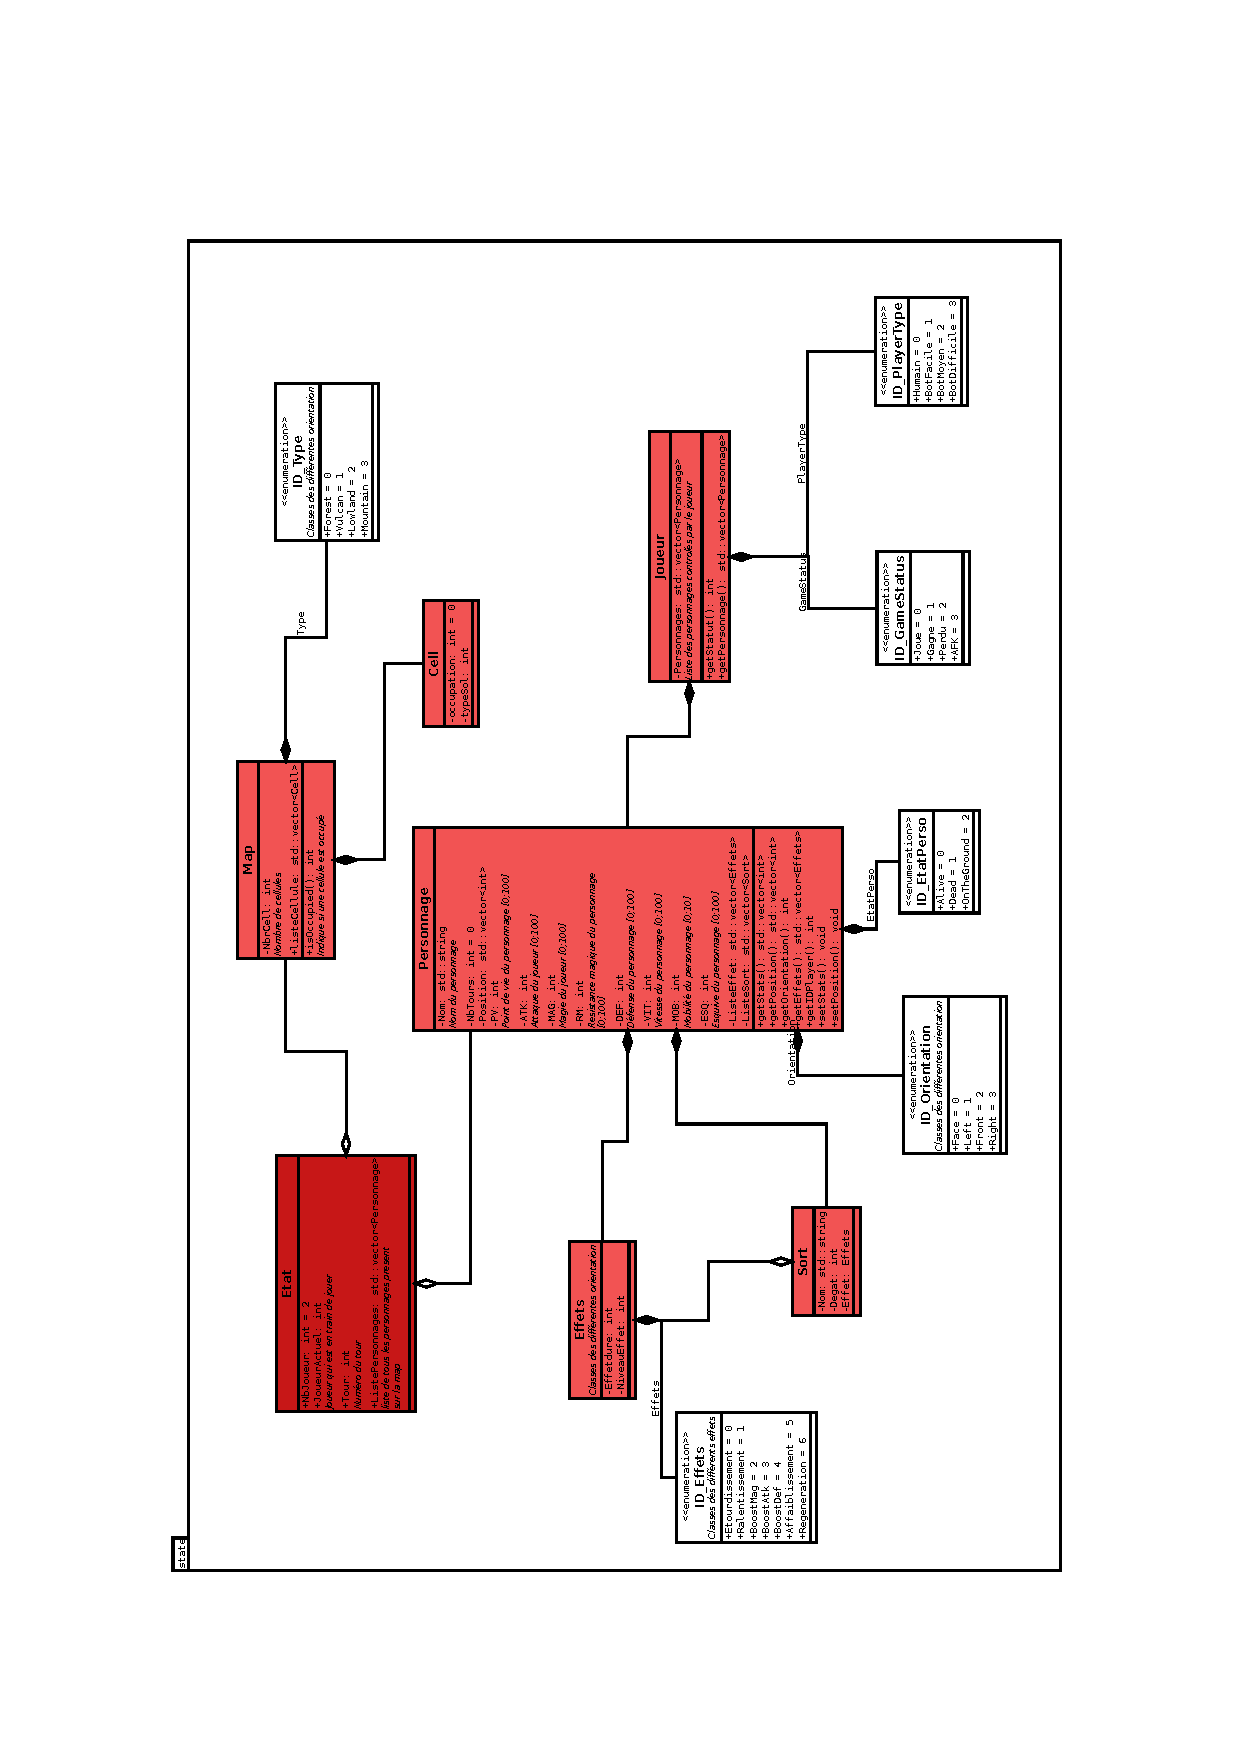
\includegraphics[width=0.8\paperwidth,angle=270]{StateUML_1.pdf}
\caption{\label{uml:state}Diagramme des classes d'état.} 
\end{figure}
\end{landscape}

\clearpage
\section{Rendu: Stratégie et Conception}

\subsection{Stratégie de rendu d'un état}


\subsection{Conception logiciel}

%\begin{landscape}
%\begin{figure}[p]
%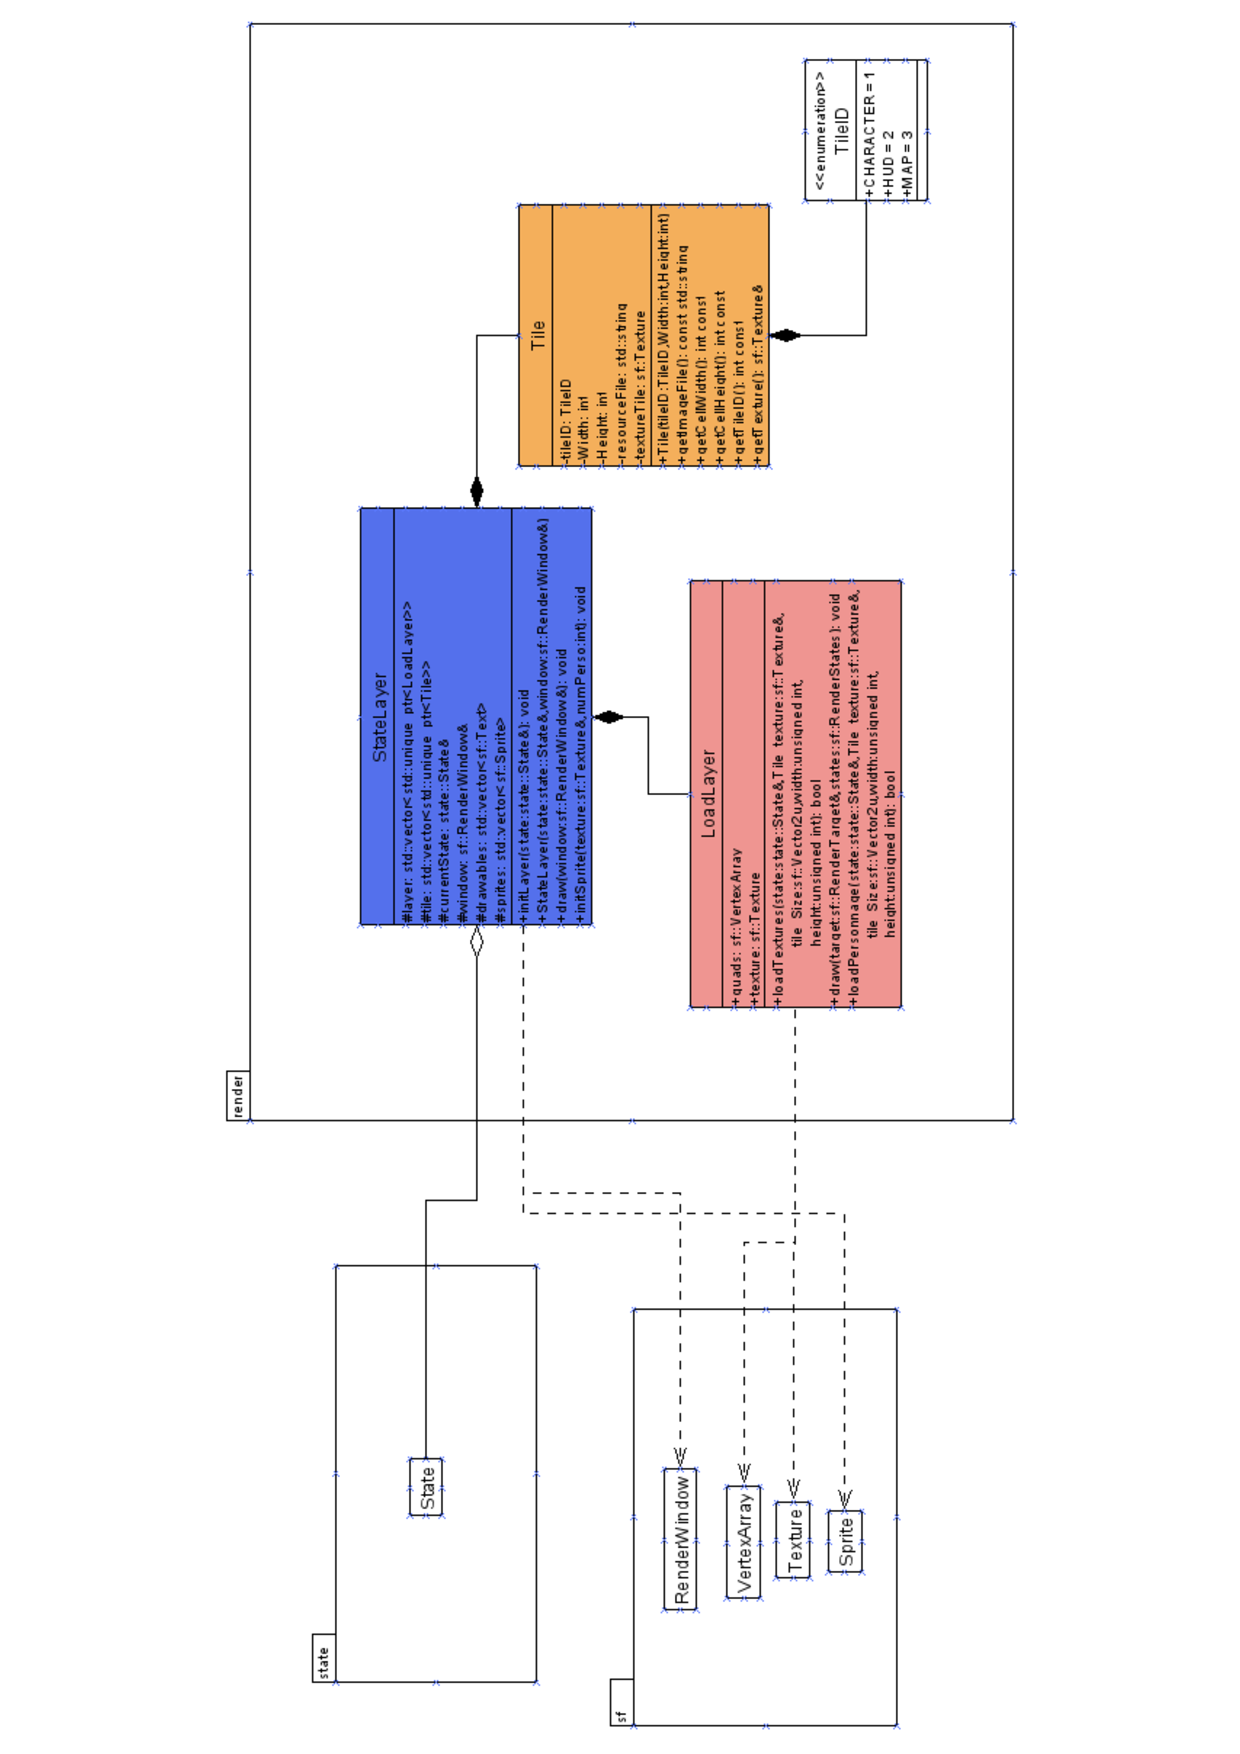
\includegraphics[width=0.9\paperheight]{render.pdf}
%\caption{\label{uml:render}Diagramme des classes de rendu.} 
%\end{figure}
%\end{landscape}

\clearpage
\section{Règles de changement d'états et moteur de jeu}

\subsection{Règles}

\subsubsection{Actualisation}

L'engine est complètement indépendant du render, le mmoteur de jeu
ne sert qu'à mettre a jour l'état du jeu, en fonction des commandes exterieurs 
(Clavier, souris ou serveur), et des règles automatiques, qui sont vérifer a chaque 
changement d'état. Le moteur de jeu effectue une mise a jour de l'état a chaque
commande exterieur, les règles autonomes n'ont besoin de s'activer qu'uniquement s'y 
il y a un changement d'état (jeu tour par tour).

\subsubsection{Règles extérieurs}

Les règles extérieurs sont provoqué par les cliques de souris a diffrénts endroit, 
ou les ordres reçue par le réseau.

\begin{itemize}
  \item Selectionner un personnage, afin d'afficher les statistiques du personnage
  \item Déplacer les personnages
  \item Attaquer un ennemi
  \item Lancer un sort
\end{itemize}

\subsubsection{Règles autonomes}

Les règles autonomes sont les checks qui sont lancés a chaque fois que l'ont veut faire
une action, afin de savoir si l'action est valide. Ainsi que la barre d'action qui détermine
l'ordre des tours.

Les différentes règles suivant les actions sont :

\begin{itemize}
  \item Tester les positions relatives des personnages
  \item Calculer les dégats d'une attaque
  \item Infliger les dégats d'une attaque 
  \item Appliquer les effets des sorts
  \item Vérifier la possibililté des déplacements
\end{itemize}

\clearpage
\subsection{Conception logiciel}

Le diagramme de classe de moteur de jeu est reprsenté sur la figure %\ref{uml:engine}.
Le jeu repose sur un patron de conception de type Command.

La classe commande est une classe abstraite qui parentes toutes les autres classe commande



%\begin{landscape}
%\begin{figure}[p]
%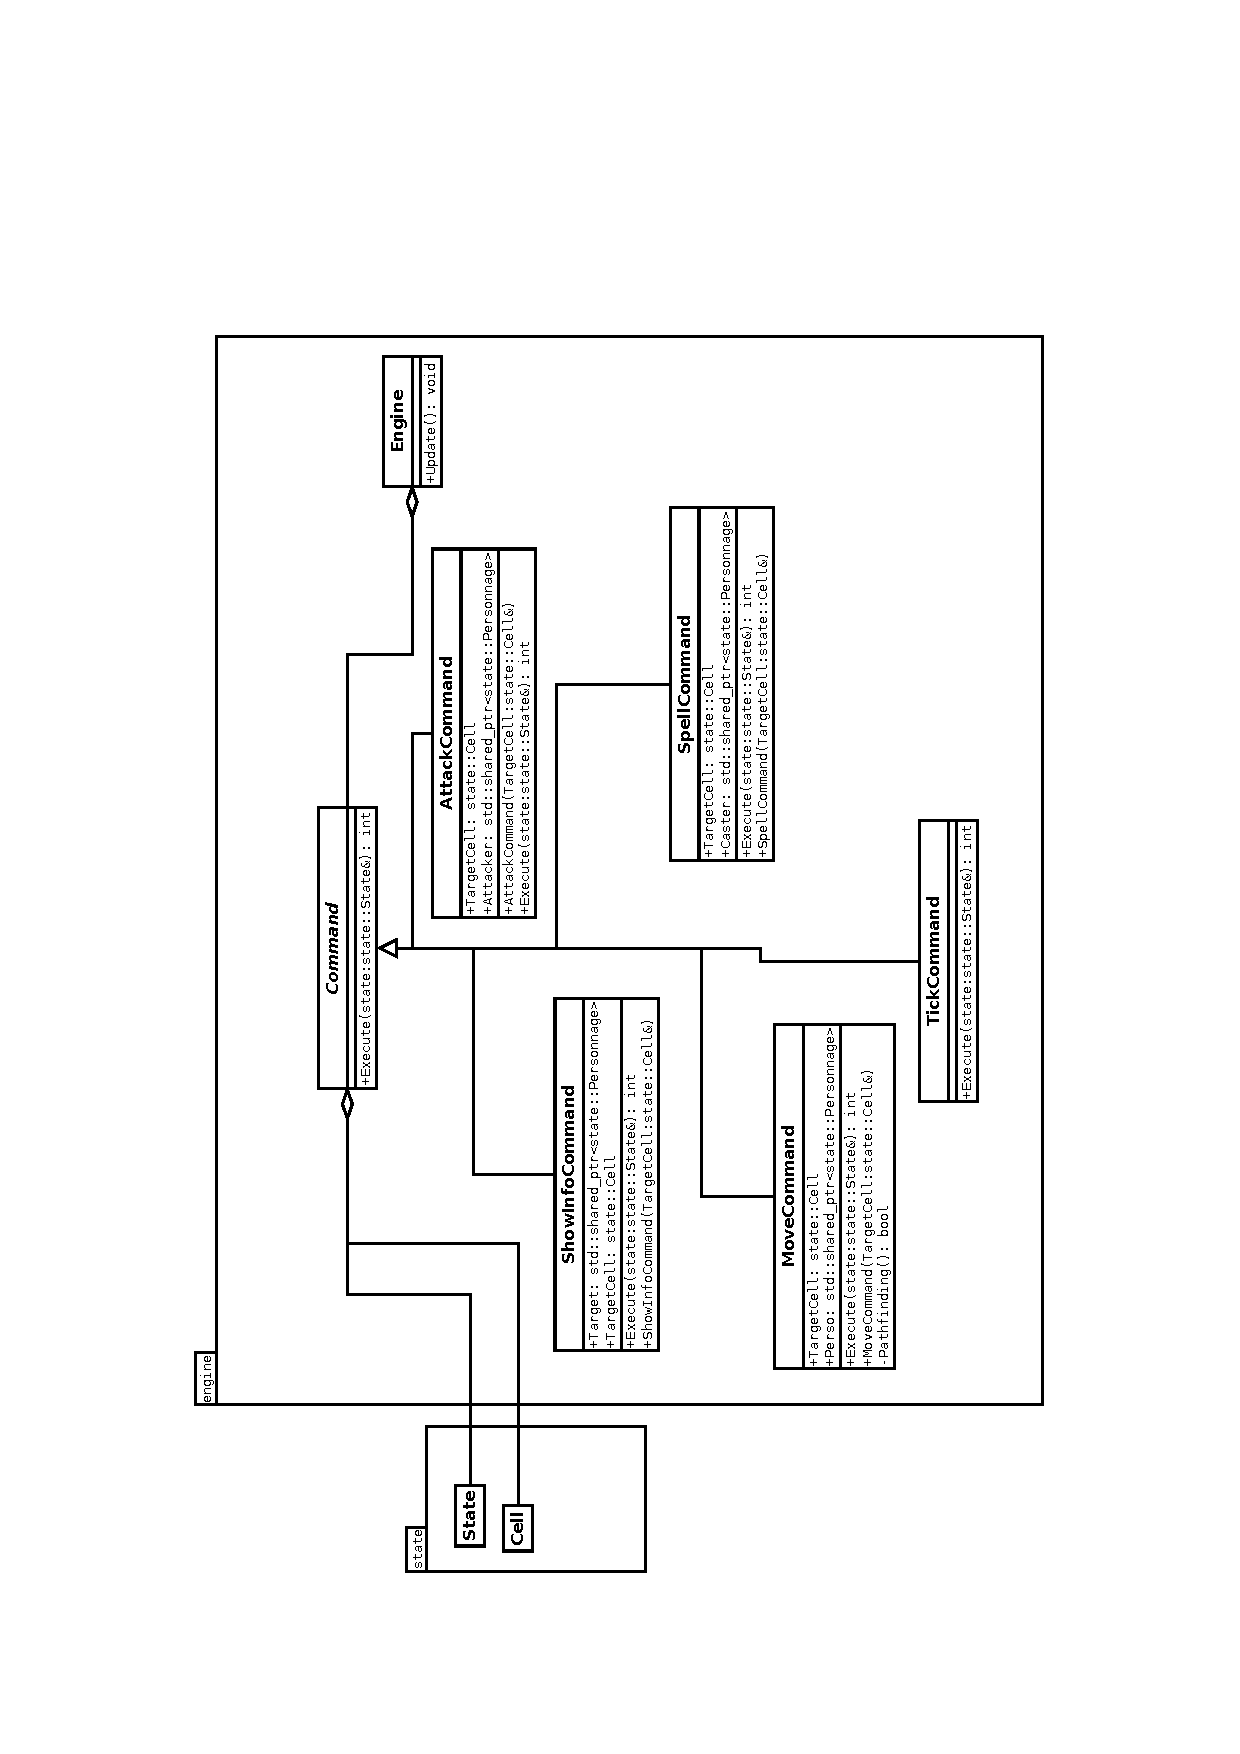
\includegraphics[width=0.9\paperheight]{engine.pdf}
%\caption{\label{uml:engine}Diagramme des classes de moteur de jeu.} 
%\end{figure}
%\end{landscape}


\section{Intelligence Artificielle}

\subsection{Stratégies}

\clearpage
\subsection{Conception logiciel}


%\begin{landscape}
%\begin{figure}[p]
%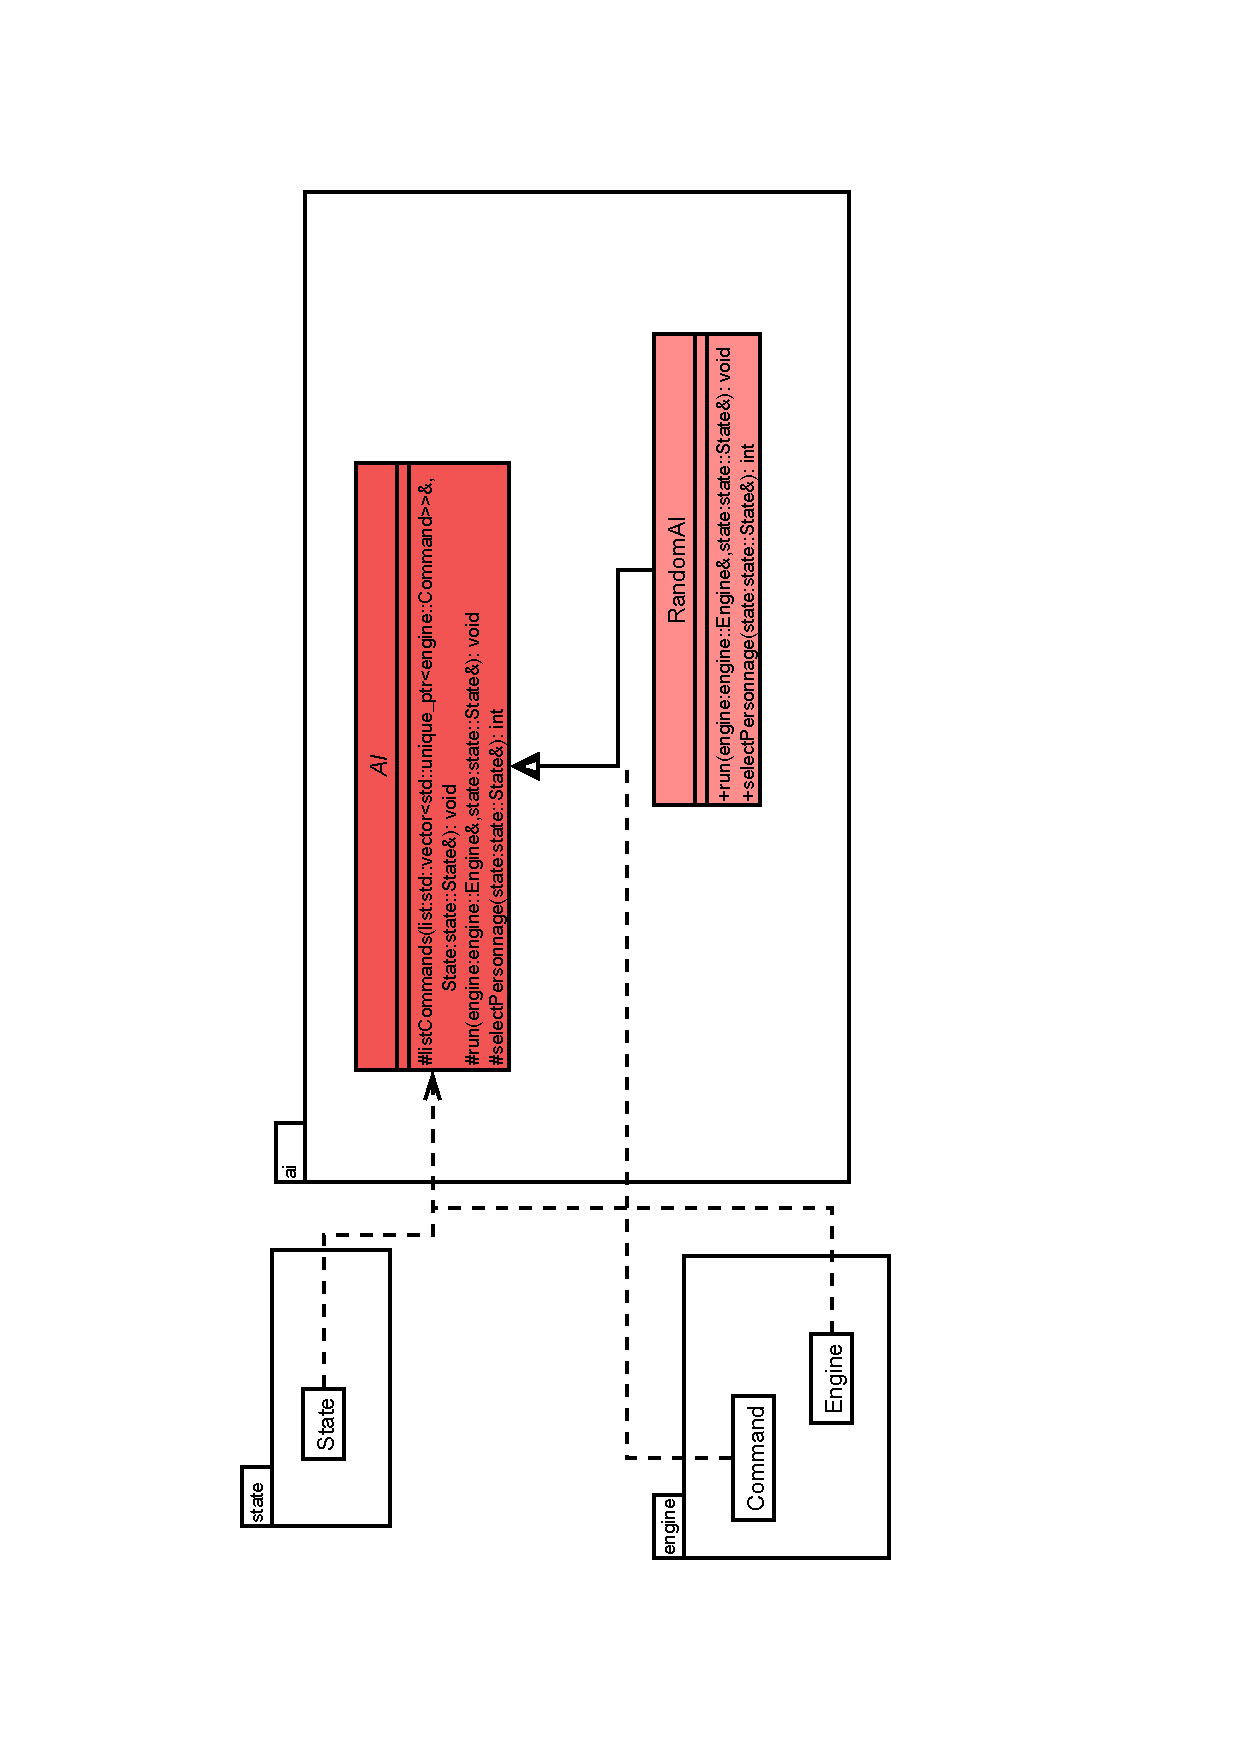
\includegraphics[width=0.9\paperheight]{ai.pdf}
%\caption{\label{uml:ai}Diagramme des classes d'intelligence artificielle.} 
%\end{figure}
%\end{landscape}


\section{Modularisation}
\label{sec:module}

\subsection{Organisation des modules}

\clearpage
\subsection{Conception logiciel}


%
%\begin{landscape}
%\begin{figure}[p]
%\includegraphics[width=0.9\paperheight]{module.pdf}
%\caption{\label{uml:module}Diagramme des classes pour la modularisation.} 
%\end{figure}
%\end{landscape}

\end{document}
